\documentclass{standalone}
\usepackage{tikz}
\usetikzlibrary{patterns, positioning}
\usepackage[sfdefault]{ClearSans} %% option 'sfdefault' activates Clear Sans as the default text font
\usepackage[T1]{fontenc}

\begin{document}
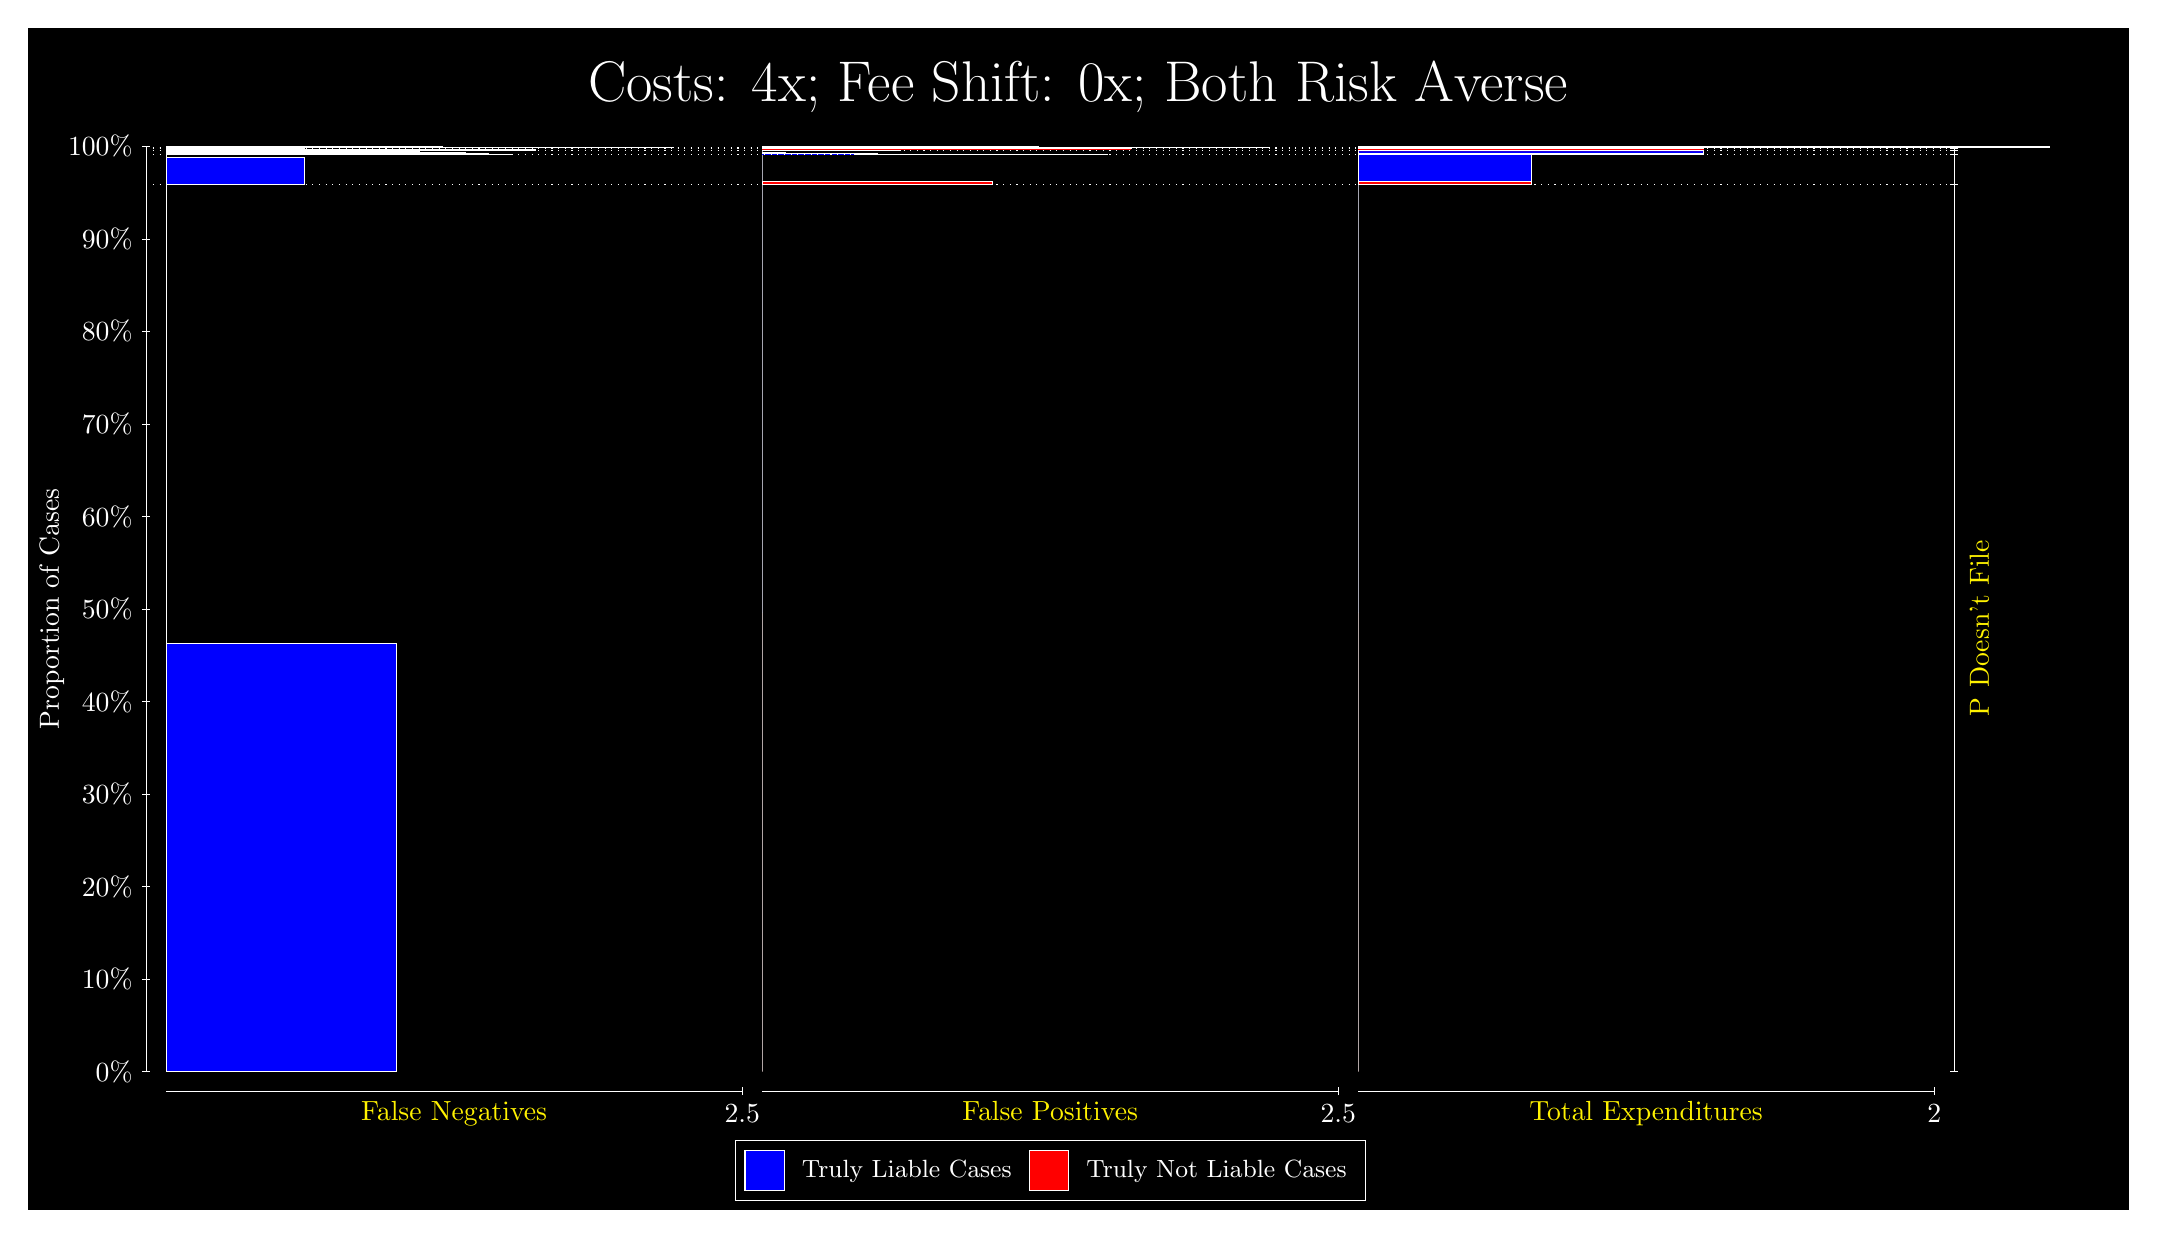
\begin{tikzpicture}
\draw[fill=black] (0,0) rectangle (26.667,15);
\draw[text=white] (0,13.5) rectangle (26.667,15) node[midway] {\huge Costs: 4x; Fee Shift: 0x; Both Risk Averse};
\draw[white, very thin] (1.5,1.75) -- (1.5,13.5);
\node[rotate=90, text=white, anchor=center] at (0.3, 7.625) {Proportion of Cases};
\draw[white, very thin] (1.45,1.75) -- (1.55,1.75);
\node[text=white, anchor=east] at (1.45, 1.75) {0\%};
\draw[white, very thin] (1.45,2.925) -- (1.55,2.925);
\node[text=white, anchor=east] at (1.45, 2.925) {10\%};
\draw[white, very thin] (1.45,4.1) -- (1.55,4.1);
\node[text=white, anchor=east] at (1.45, 4.1) {20\%};
\draw[white, very thin] (1.45,5.275) -- (1.55,5.275);
\node[text=white, anchor=east] at (1.45, 5.275) {30\%};
\draw[white, very thin] (1.45,6.45) -- (1.55,6.45);
\node[text=white, anchor=east] at (1.45, 6.45) {40\%};
\draw[white, very thin] (1.45,7.625) -- (1.55,7.625);
\node[text=white, anchor=east] at (1.45, 7.625) {50\%};
\draw[white, very thin] (1.45,8.8) -- (1.55,8.8);
\node[text=white, anchor=east] at (1.45, 8.8) {60\%};
\draw[white, very thin] (1.45,9.975) -- (1.55,9.975);
\node[text=white, anchor=east] at (1.45, 9.975) {70\%};
\draw[white, very thin] (1.45,11.15) -- (1.55,11.15);
\node[text=white, anchor=east] at (1.45, 11.15) {80\%};
\draw[white, very thin] (1.45,12.325) -- (1.55,12.325);
\node[text=white, anchor=east] at (1.45, 12.325) {90\%};
\draw[white, very thin] (1.45,13.5) -- (1.55,13.5);
\node[text=white, anchor=east] at (1.45, 13.5) {100\%};

\draw[white, very thin] (24.457,1.75) -- (24.457,13.5);
\draw[white, very thin] (24.407,1.75) -- (24.507,1.75);
\node[anchor=west] at (24.407, 1.75) {};
\draw[white, very thin] (24.407,13.013) -- (24.507,13.013);
\node[anchor=west] at (24.407, 13.013) {};
\draw[white, very thin] (24.407,13.4) -- (24.507,13.4);
\node[anchor=west] at (24.407, 13.4) {};
\draw[white, very thin] (24.407,13.45) -- (24.507,13.45);
\node[anchor=west] at (24.407, 13.45) {};
\draw[white, very thin] (24.407,13.47) -- (24.507,13.47);
\node[anchor=west] at (24.407, 13.47) {};
\draw[white, very thin] (24.407,13.488) -- (24.507,13.488);
\node[anchor=west] at (24.407, 13.488) {};
\draw[white, very thin] (24.407,13.49) -- (24.507,13.49);
\node[anchor=west] at (24.407, 13.49) {};
\draw[white, very thin] (24.407,13.5) -- (24.507,13.5);
\node[anchor=west] at (24.407, 13.5) {};

\draw[white, very thin, fill=blue] (1.75,1.75) rectangle (4.6775,7.1894);
\draw[white, very thin, fill=red] (1.75,7.1894) rectangle (1.75,13.013);
\draw[white, very thin, fill=blue] (1.75,13.013) rectangle (3.5065,13.359);
\draw[white, very thin, fill=red] (1.75,13.359) rectangle (1.75,13.4);
\draw[white, very thin, fill=blue] (1.75,13.4) rectangle (6.1413,13.403);
\draw[white, very thin, fill=blue] (1.75,13.403) rectangle (5.8486,13.409);
\draw[white, very thin, fill=blue] (1.75,13.409) rectangle (5.5558,13.423);
\draw[white, very thin, fill=blue] (1.75,13.423) rectangle (5.2631,13.427);
\draw[white, very thin, fill=blue] (1.75,13.427) rectangle (4.9703,13.433);
\draw[white, very thin, fill=blue] (1.75,13.433) rectangle (4.6775,13.438);
\draw[white, very thin, fill=blue] (1.75,13.438) rectangle (4.3848,13.441);
\draw[white, very thin, fill=blue] (1.75,13.441) rectangle (4.092,13.443);
\draw[white, very thin, fill=blue] (1.75,13.443) rectangle (3.7993,13.444);
\draw[white, very thin, fill=red] (1.75,13.444) rectangle (1.75,13.45);
\draw[white, very thin, fill=blue] (1.75,13.45) rectangle (6.4341,13.468);
\draw[white, very thin, fill=red] (1.75,13.468) rectangle (1.75,13.47);
\draw[white, very thin, fill=blue] (1.75,13.47) rectangle (3.5065,13.487);
\draw[white, very thin, fill=red] (1.75,13.487) rectangle (1.75,13.488);
\draw[white, very thin, fill=blue] (1.75,13.488) rectangle (8.1906,13.489);
\draw[white, very thin, fill=red] (1.75,13.489) rectangle (1.75,13.49);
\draw[white, very thin, fill=blue] (1.75,13.49) rectangle (5.2631,13.499);
\draw[white, very thin, fill=red] (1.75,13.499) rectangle (1.75,13.5);
\draw[white, very thin, fill=red] (9.3189,1.75) rectangle (9.3189,7.5739);
\draw[white, very thin, fill=blue] (9.3189,7.5739) rectangle (9.3189,13.013);
\draw[white, very thin, fill=red] (9.3189,13.013) rectangle (12.246,13.054);
\draw[white, very thin, fill=blue] (9.3189,13.054) rectangle (9.3189,13.4);
\draw[white, very thin, fill=red] (9.3189,13.4) rectangle (13.71,13.4);
\draw[white, very thin, fill=red] (9.3189,13.4) rectangle (13.417,13.4);
\draw[white, very thin, fill=red] (9.3189,13.4) rectangle (13.125,13.4);
\draw[white, very thin, fill=red] (9.3189,13.4) rectangle (12.832,13.401);
\draw[white, very thin, fill=red] (9.3189,13.401) rectangle (12.539,13.401);
\draw[white, very thin, fill=red] (9.3189,13.401) rectangle (12.246,13.402);
\draw[white, very thin, fill=red] (9.3189,13.402) rectangle (11.954,13.403);
\draw[white, very thin, fill=red] (9.3189,13.403) rectangle (11.661,13.404);
\draw[white, very thin, fill=red] (9.3189,13.404) rectangle (11.368,13.405);
\draw[white, very thin, fill=blue] (9.3189,13.405) rectangle (10.783,13.406);
\draw[white, very thin, fill=blue] (9.3189,13.406) rectangle (10.49,13.408);
\draw[white, very thin, fill=blue] (9.3189,13.408) rectangle (10.197,13.411);
\draw[white, very thin, fill=blue] (9.3189,13.411) rectangle (9.9044,13.416);
\draw[white, very thin, fill=blue] (9.3189,13.416) rectangle (9.6116,13.423);
\draw[white, very thin, fill=blue] (9.3189,13.423) rectangle (9.3189,13.45);
\draw[white, very thin, fill=red] (9.3189,13.45) rectangle (11.075,13.452);
\draw[white, very thin, fill=blue] (9.3189,13.452) rectangle (9.3189,13.47);
\draw[white, very thin, fill=red] (9.3189,13.47) rectangle (14.003,13.472);
\draw[white, very thin, fill=blue] (9.3189,13.472) rectangle (11.075,13.488);
\draw[white, very thin, fill=red] (9.3189,13.488) rectangle (12.832,13.489);
\draw[white, very thin, fill=blue] (9.3189,13.489) rectangle (9.9044,13.49);
\draw[white, very thin, fill=red] (9.3189,13.49) rectangle (15.759,13.491);
\draw[white, very thin, fill=blue] (9.3189,13.491) rectangle (12.832,13.5);
\draw[white, very thin, fill=red] (16.888,1.75) rectangle (16.888,7.5739);
\draw[white, very thin, fill=blue] (16.888,7.5739) rectangle (16.888,13.013);
\draw[white, very thin, fill=red] (16.888,13.013) rectangle (19.083,13.054);
\draw[white, very thin, fill=blue] (16.888,13.054) rectangle (19.083,13.4);
\draw[white, very thin, fill=red] (16.888,13.4) rectangle (21.279,13.4);
\draw[white, very thin, fill=blue] (16.888,13.4) rectangle (21.279,13.406);
\draw[white, very thin, fill=red] (16.888,13.406) rectangle (21.279,13.41);
\draw[white, very thin, fill=blue] (16.888,13.41) rectangle (21.279,13.444);
\draw[white, very thin, fill=red] (16.888,13.444) rectangle (21.279,13.444);
\draw[white, very thin, fill=blue] (16.888,13.444) rectangle (21.279,13.45);
\draw[white, very thin, fill=red] (16.888,13.45) rectangle (21.279,13.452);
\draw[white, very thin, fill=blue] (16.888,13.452) rectangle (21.279,13.47);
\draw[white, very thin, fill=red] (16.888,13.47) rectangle (21.279,13.472);
\draw[white, very thin, fill=blue] (16.888,13.472) rectangle (21.279,13.488);
\draw[white, very thin, fill=red] (16.888,13.488) rectangle (25.67,13.489);
\draw[white, very thin, fill=blue] (16.888,13.489) rectangle (25.67,13.49);
\draw[white, very thin, fill=red] (16.888,13.49) rectangle (25.67,13.491);
\draw[white, very thin, fill=blue] (16.888,13.491) rectangle (25.67,13.5);
\draw[white, dotted] (1.5,13.013) -- (24.457,13.013);
\draw[white, dotted] (1.5,13.4) -- (24.457,13.4);
\draw[white, dotted] (1.5,13.45) -- (24.457,13.45);
\draw[white, dotted] (1.5,13.47) -- (24.457,13.47);
\draw[white, dotted] (1.5,13.488) -- (24.457,13.488);
\draw[white, dotted] (1.5,13.49) -- (24.457,13.49);
\draw[white, very thin] (1.75,1.5) -- (9.0689,1.5);
\node[text=yellow, anchor=north] at (5.4094, 1.5) {False Negatives};
\draw[white, very thin] (9.0689,1.45) -- (9.0689,1.55);
\node[text=white, anchor=north] at (9.0689, 1.45) {2.5};

\draw[white, very thin] (9.3189,1.5) -- (16.638,1.5);
\node[text=yellow, anchor=north] at (12.978, 1.5) {False Positives};
\draw[white, very thin] (16.638,1.45) -- (16.638,1.55);
\node[text=white, anchor=north] at (16.638, 1.45) {2.5};

\draw[white, very thin] (16.888,1.5) -- (24.207,1.5);
\node[text=yellow, anchor=north] at (20.547, 1.5) {Total Expenditures};
\draw[white, very thin] (24.207,1.45) -- (24.207,1.55);
\node[text=white, anchor=north] at (24.207, 1.45) {2};

\node[text=yellow, centered, rotate=90] at (24.777, 7.3816) {P Doesn't File};







\draw (12.978300999999998,1.5) node[draw=none] (baseCoordinate) {};
\begin{scope}[align=center]
        \matrix[scale=0.5, draw=white, below=0.5cm of baseCoordinate, nodes={draw}, column sep=0.1cm]{
            \node[rectangle, draw, minimum width=0.5cm, minimum height=0.5cm, fill=blue] {}; &
            \node[draw=none, font=\small, text=white] (B) {Truly Liable Cases}; &
            \node[rectangle, draw, minimum width=0.5cm, minimum height=0.5cm, fill=red] {}; &
            \node[draw=none, font=\small, text=white] (B) {Truly Not Liable Cases}; \\
            };
\end{scope}

\end{tikzpicture}
\end{document}